% !TEX encoding = UTF-8 Unicode
% !TEX program = pdflatex
% !TEX spellcheck = en_US


% In order to correctly compile this document,
% execute the following commands:
% 1. pdflatex
% 2. pdflatex
% 3. pdflatex



\documentclass[amsthm,ebook]{saparticle}

% IF YOU USE PDFLATEX
\usepackage[utf8x]{inputenc}
% if you write in english and in greek
\usepackage{ucs}
\usepackage[greek,english]{babel}
\languageattribute{greek}{polutoniko}

% IF YOU USE XELATEX
%\usepackage{polyglossia}
% if you write in italian
%\setmainlanguage{italian}
% If you want put some ancient greek:
%\setotherlanguage[variant=polytonic]{greek}
%\newfontfamily{\greekfont}[Ligatures=TeX]{Palatino Linotype}

% dummy text (remove in a normal thesis)
% remove if not necessary
\usepackage{siunitx}
%Natbib for bibliography management
\usepackage[authoryear]{natbib}
% custom commands
\newcommand{\bs}{\textbackslash}

%%%%%%%%
%TITLE:%
%%%%%%%%
\title{Deixis and Frames of Reference in Dedicatory Epigrams. 
The use of a database with an interdisciplinary approach}
\author[topoi]{Flavia Licciardello\corref{first}}
\address[topoi]{Humboldt Universität zu Berlin, Excellence Cluster TOPOI}
\cortext[first]{Corresponding author. Email: flavia.licciardello@topoi.org}
\date{2015-11-20}
\begin{document}

\maketitle
\begin{abstract}
This paper presents an example of a database designed to combine epigraphic, linguistic and philological data. This database is part of my project on a study of deictic expressions in dedicatory inscribed and
literary epigrams. It includes the results of the analysis of around 600 dedicatory epigrams and it will be used to
extract information on trends and recurrent patterns in the genre.
\end{abstract}
\keywords{Greek epigram, dedication, database, deixis, Hellenistic age}

\section{Introduction}


\noindent For a long time, the study of the Greek epigrams has maintained a clear distinction between `epigraphic' and `literary'
epigrams. This distinction, however, fails to understand the complexity and the development of this poetic genre. Only
in very recent years have scholars started to highlight properly the important relationship between Hellenistic
`literary' epigrams and epigraphic models.\footnote{ The shift in the attitude towards the history of the epigrammatic
genre is well resumed by \citep[5-34]{garulli_byblos_2012}. For other work, which consider the importance of the dialogue between
`epigraphic' and `literary' epigrams, see e.g. \citep{meyer_inszeniertes_2005}, \citep{tueller_look_2008}. On archaic and classical epigrams, see
\citep{baumbach_archaic_2010}. Further bibliography in \citep[2]{baumbach_archaic_2010}.} 

My PhD project follows this new exegetic line and contributes to our understanding of the inscriptional component of the
Hellenistic epigram.\footnote{ The project is developed within the frame of the C-1 group (`Deixis and frame of
reference) of the Excellence Cluster TOPOI.} In particular, I focus on the use of deictic expressions in dedicatory
epigrams, i.e. on the use of all those linguistic elements whose meaning and interpretation depend on the spatial and
temporal context where they are uttered.\footnote{ For an overview of the concept of deixis see \citet[with further bibliography)]{diessel_deixis_2012}. On deixis in Ancient Greek see e.g. \citet{felson_poetics_2004}, \citet{edmunds_deixis_2008} and \citep{bonifazi_deixis_2014}.} The
corpus analysed includes inscribed epigrams from the archaic epoch until the end of the 4th century BC, and the
Hellenistic epigrams transmitted in the Greek Anthology or on papyrus. The reference editions used are \citep[1-2]{hansen_carmina_1983}
for inscribed epigrams and \citep{gow_greek_1965} and \citep{austin_posidippi_2002} for `literary epigrams'.\footnote{ For
convenience, I will later on refer to this second group as `literary epigrams'. The definition simply identifies those
epigrams that are transmitted in the Greek Anthology or on papyrus and does not imply any value judgment.} 

In order to deal with this heterogeneous material, I developed a database to register and organise the data obtained
from the analysis of the texts. The specific aim of this database is the registration of all relevant linguistic
features related to spatial, personal and temporal deixis. In addition to this, I put on record for each epigram other
more generic elements, which are related to the dedicatory context, to the linguistic facies and, especially in the
case of inscribed epigrams, to the historical and archaeological context. In this way, on the one hand, I can obtain a
global picture of the whole corpus, which includes data found both in inscribed and literary epigrams. At the same
time, I can keep and easily retrieve all the peculiar features related to each specific text in order to be able to
deal with the material properly, without losing sight of their specificity. The possibility of managing at the same
time these two levels - the whole corpus and the single text – is extremely valuable. In this regard, the database
provides an essential support, since it helps work with complex material on those different levels that must be
considered together, but are usually difficult to keep in focus at the same time.




\section{Greek dedicatory epigrams and the role of deixis}


\noindent In the Ancient Greek world it was customary to accompany a dedication to the gods with a – usually – short inscription.
This was normally chiselled on the dedicated object (or on its support) and it recorded the main information related to
the offering. The elements recurring in such inscriptions were the name of the dedicator, the verb of dedication and
the name of the god receiving the dedication.\footnote{ On archaic dedications, see \citet[spec. 1-14]{day_archaic_2010} for
an introduction to the genre.} The most common and widespread formula for dedications contained exactly these three
elements: \begin{otherlanguage*}{greek}ὁ δεῖνα ἀνέθηκε τῷ θεῷ\end{otherlanguage*}. A frequent variation was \begin{otherlanguage*}{greek}ὁ δεῖνά με ἀνέθηκε τῷ θεῷ\end{otherlanguage*}, \footnote{ The formula here presented (with its two variants) was \ identified by Maria Letizia Lazzarini, in
her study on the formulas of archaic dedications \citet[58-60]{lazzarini_formule_1976}. Her analysis is based on both verse and prose
inscriptions from the archaic age. However, such basic scheme, with these elements, was normal in epigrams as well and
it remained substantially unchanged in classical and post-classical time.} \ where the speaker is the object itself, as
is clear from the employment of the personal pronoun \begin{otherlanguage*}{greek}με\end{otherlanguage*}. It is interesting to note that since their first
examples the speaking object was a recurring feature in dedicatory epigrams and it is still frequent in the 4th century
BC.\footnote{ On the topos of the speaking object, see \citet{burzachechi_oggetti_1962}, \citet[36-52]{svenbro_phrasikleia:_1988}, \citet[16-27]{tueller_look_2008}, \citet[151-166]{furley_life_2010}, \citet[250-260]{wachter_origin_2010}, \citet[29-107]{christian_gebildete_2014}.} Clearly, the basic scheme here
presented could be varied by omitting some elements (as the name of the dedicator) or adding others (as the generic
name of the object, like the recurrent \begin{otherlanguage*}{greek}ἄγαλμα\end{otherlanguage*}).

A crucial moment in the evolution of the epigrammatic genre is the beginning of the Hellenistic era, when the genre becomes more and more popular and epigrams started to be circulated autonomously, no longer limited to one
inscription alone.\footnote{ This trend may be linked to the custom prevalent in the 5th and 4th century BC to copy
epigrams on monuments and then quote them in various texts. See \citet[47ff.]{gutzwiller_poetic_1998}} This development led to the
composition of literary epigrams not intended for inscription, but which in some way maintained the illusion of a
material inscription on a stone. The Hellenistic epigrammatists who worked with inscriptional type of epigrams (and
among these dedicatory epigrams) retained the structure, style and traditions of the epigraphic models, yet the
translation of these into a book context inevitably means that the communicative strategies employed until then had to
be reinvented. The primary reason for such changes is self-evident: the monument intended for inscription and the space
surrounding it do not exist anymore – they have to be imagined in the reader's mind.\footnote{ This involvement of the
reader can be put in relation with what \citet{Bing1995} defines Ergänzungsspiel, i.e. with the process of supplementation
of the text deliberately incited by Hellenistic epigrammatists.}

This process of reinvention is particularly evident in dedicatory epigrams, which were traditionally chiselled on the
dedicated object itself. In this case, the loss of the original context forces the author to re-elaborate traditional
models, by adding some elements (e.g. the specific name of the dedicated object) that cannot be retrieved from the
surrounding setting. 

From a linguistic point of view, this re-elaboration has an impact in the texts on deictic expressions, which were
typically used in inscriptions to lead the gaze of the reader towards the dedicated object. In this epigraphic context
the deictic expressions point to something in front of reader's eyes (deixis ad oculos), whereas in a literary context
the readers will have to imagine in their mind the invisible referents of deictic expressions (deixis am
Phantasma).\footnote{ The difference between deixis ad oculos and deixis am Phantasma was highlighted and described for
the first time by Bühler in 1934, see \citet[121-126, 133-135]{buhler_sprachtheorie:_1982}.} If on the one hand this change requires a
particular attention to the verbal reconstruction of the setting, on the other hand, the loss of the material context
allows the poet to play with different and new points of view and frames of reference. 

The analysis of deictic expressions can help determine the deictic centre in dedicatory epigrams. The deictic
centre, which normally coincides with the origin of the utterance, works as a point of reference for all deictic
markers and expression.\footnote{See \citet[102f.]{buhler_sprachtheorie:_1982} and \citet[63f.]{levinson_pragmatics_1983}.} In the case of dedicatory
epigrams on stone, the deictic centre in spatial terms is generally understood to be in the place of the inscription
itself, which in most cases is the dedicated object. In other words, for all deictic expressions that point to
something close (such as the proximal \begin{otherlanguage*}{greek}ὅδε\end{otherlanguage*} this here'\footnote{ `Proximal' deictic elements are all those
elements that refers to something that is close to the deictic centre: among these demonstrative pronouns or adverbs such as `this' or `here' and
temporal adverbs such as `now'. See \citet[2408f.]{diessel_deixis_2012}.}) the occasional reader will look for the referents in the
space close to the inscription. In the evolution of the epigrammatic genre, the loss of the material context produces
an important change, since the strong relation that connects the text with its object starts to fade. In other words, when the epigram is found in a book, the point of reference --- or deictic centre --- is not immediately clear to the reader, since it is not immediately clear the relation of the text with the spatial setting to which it refers.  This means that
the deictic centre is somehow released from its traditional location on the object and the poet is free to consider and
bring to the text new, different points of view. 

This progressive detachment of the text from its original physical location played a crucial role in the process
that led, out of trivial verse inscriptions, to the emergence of the epigram as a full literary genre. Deictic
expressions were traditionally employed in epigraphic contexts to strictly and clearly bind the text to its material
support. Later on, only the possibility of the separation from a unique location allows the epigram to be circulated
autonomously and reach a wider audience. In this passage, poets explore new uses of deictic markers in order to
widen the possible references of their text. 

My research will try to detect different trends in the use of deictic expressions in order to highlight the similarities
and parallelisms between inscribed and literary epigrams and to elucidate the different deictic strategies employed in
different contexts.

\section{The database}


\noindent In the first step of my research, the analysis of the texts is followed by the registration into a database of all the
relevant data related to spatial, personal and temporal deixis. This database is conceived first of all as a tool to
organise the data and make them available for the next steps of the research.

The corpus of epigrams analysed includes dedicatory verse-inscriptions collected in Hansen's Carmina Epigraphica Graeca
[CEG 1-2], as for epigrams on stone. In this case, I selected those epigrams included by Hansen in the section ``Tituli
dedicatorii''. For literary epigrams, I followed Gow's and Page's edition \citep{gow_greek_1965}, to which I added
the epigrams attributed to Posidippus and edited by Austin and Bastianini \citep{austin_posidippi_2002}. In this case, the
selection was made according to the contents of the epigrams and I selected all those epigrams that have a clear
dedicatory frame.

The structure of the database was designed to include all important data related to the text examined, in order to have
for each epigram a complete profile, which includes linguistic, literary, historical and archaeological
aspects.\footnote{ The software used is FileMaker Pro 13.0v4.} The data were organised in various tables, which are all interconnected (See Fig.~\ref{fig:1}). 

\begin{figure}[!bp]
\centering
 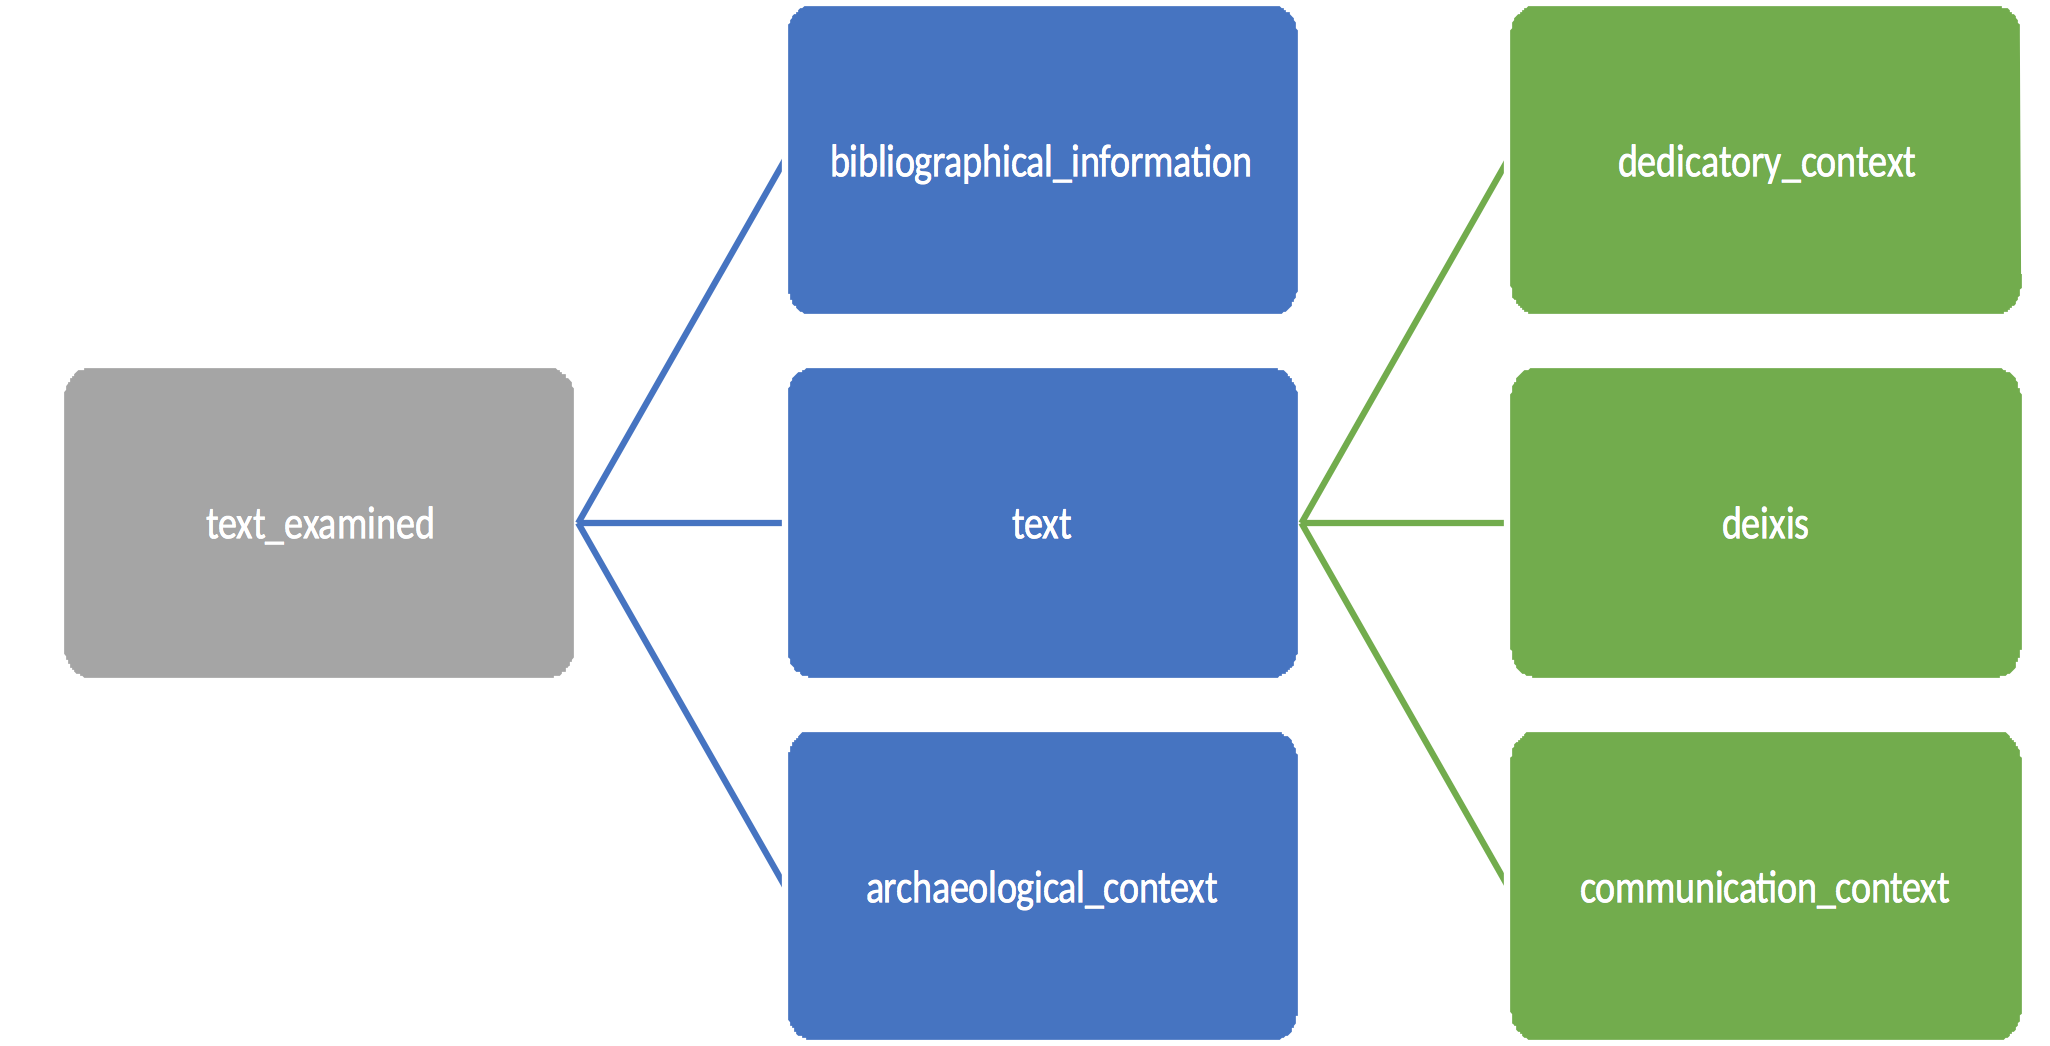
\includegraphics[width=\columnwidth]{schema.png}
\caption{default}
\label{fig:1}
\end{figure}


Alongside bibliographical and historical-archaeological information, the database records the data obtained by a first
analysis of the form and of linguistic features of the epigram, such as verbal tenses, occurrences of demonstrative and
personal pronouns (deixis); speaking subject and addressee (communicative\_context); verb of dedication, standard name
of the dedicated object (dedicatory\_context).
Such structure offers a balance between the need to record a detailed picture for each epigram analysed and the
possibility of conducting research on single features within the whole corpus. Since each table contains a restricted
amount of data (divided into coherent sections), it is easy to get a simple, clear picture of the recurrence of one
specific feature (and its interconnection with other related aspects) within the corpus and to leave out information
that is not immediately consistent with the research done. However, the fact that all the tables are interconnected enables the user to formulate queries that combine fields contained in different tables. In this way, for example, it is possible to look for the
recurrence of a specific tense for the verb of dedication (in the table `deixis') and to see if this is associated with
the use of a specific verb of dedication (in the table `dedicatory\_context') or with a particular epoch (in the table
`archeological\_context').




\section{An example: the present tense in dedicatory epigrams}


\noindent The verbal tenses can work as temporal deictic markers and can play an important role in the definition of the temporal
frame.\footnote{ Though the grammatical category of tense does not always coincide with the semantic category of time,
it is still possible to retrace in the use of a peculiar verbal form a reference to time. However, such analysis must
always consider other linguistic elements, which contribute determine the temporal frame of the text. On temporal
deixis and verbal tense see \citet[677-690]{lyons_semantics_1977}; \citet[73-79]{levinson_pragmatics_1983}; \citet[14-26 and 120-130]{klein_time_1994}. For the
analysis of temporal deixis in Ancient Greek texts see e.g. \citet{dalessio_past_2004} and \citet[8f.]{edmunds_deixis_2008} (with further
bibliography).} In particular, the present tense usually decodes the present time, which is the time of the deictic
centre (`now'). Since the deictic centre operates as a point of reference for the spatial and temporal orientation,
individuating the deictic centre helps determine the frame of reference of the epigram. This could lay, for example, in
the act of dedication celebrated, in the moment of the composition by the poet or in the moment of reading.\footnote{
On the relation between the temporal frame of the utterance and the deictic centre, see \citet[79f.]{levinson_pragmatics_1983} and
\citet{dalessio_past_2004}.} \ 

In the definition of the deictic centre in dedicatory epigrams, the analysis of the verb of dedication is particularly
relevant, since this makes clear the relation of the text to the dedicatory act, which is the main piece of information
of the epigram. The most common dedicatory formula presents the verb in the indicative aorist (with augment). Leaving
aside the formulaic aorist and those cases where the verb is not expressed or lost, we find in the corpus analysed a
significant number of cases where the verb that expresses the dedication is in the indicative present.\footnote{ More
specifically, out of a corpus of 598 epigrams analysed, for the verb of dedication the aorist appears 379 times, the
present 50 times. In 172 epigrams the verb is lost or absent. Moreover, some epigrams contains more then one verb of
dedication and these could be expressed in different aspects and moods. } 

As for the 41 occurrences of verbs of dedication in the indicative present, a clear distinction can be observed between
epigrams on stone and epigrams with a literary tradition. In the first group, the present form is much more sporadic.
Out of 422 epigrams analysed, we find only 5 clear examples, from different epochs and geographical areas: [CEG 192i]
(Athens, ca. 520? BC \begin{otherlanguage*}{greek}ἀνακειμα[ι]\end{otherlanguage*}), [CEG 302] (Attica, found in Ptoion, ca. 540? BC v. 1
\begin{otherlanguage*}{greek}εἰμ᾿\end{otherlanguage*})\footnote{ For the verb \begin{otherlanguage*}{greek}εἰμί\end{otherlanguage*} in dedicatory formulas, see \citet[59f.]{lazzarini_formule_1976}.} [CEG
251] (Athens, ca. 500-480? BC v.1 \begin{otherlanguage*}{greek}εἰμὶ\end{otherlanguage*}), [CEG 390] (Apollonia Illyrica, found in Olympia, ca. 450-440? BC
v.1 \begin{otherlanguage*}{greek}ἀ̣νακείμεθα\end{otherlanguage*}), [CEG 822] (Geronthrai, 4th cent.? BC v.1
\begin{otherlanguage*}{greek}ἀνάκειται\end{otherlanguage*}).\footnote{ In addition to these, in [CEG 347] and [CEG 775i], the verbs
\begin{otherlanguage*}{greek}ἀνακείμ]εθα\end{otherlanguage*} and \begin{otherlanguage*}{greek}κοσ]μοῦμεν\end{otherlanguage*} respectively are supplied. In [CEG 830ii] the verb
\begin{otherlanguage*}{greek}ἀνάκειται\end{otherlanguage*} refers to another dedication, not to the one celebrated by the epigram.} In all these cases,
the grammatical subject of the verb is the dedicated object. The use of the present form refers therefore to the
present of the object, which, since the dedication, is for the time being in the place of the dedication. As is also
clear from the fact that in most of these cases the object is the speaker, the use of the present verb indicates that
the deictic centre is the dedicated object. It is also interesting to notice that most of the aforementioned epigrams
contain a second verb of dedication, in the formulaic aorist form.\footnote{ The exceptions are [CEG 822] and the
fragmentary [CEG 192i].} 

For Hellenistic epigrams of literary tradition, the picture is different. First, the occurrence of dedicatory verbs in
indicative present is less sporadic. Out of 176 epigrams analysed, the present form appears in 33 epigrams. In some of
these cases, the situation is similar to that found in dedications on stone: the subject of the present verb is the
dedicated object, which lays in the temporal deictic centre.\footnote{ However, as opposed to the examples found in
dedications on stone, the object is rarely the speaker. It is also interesting to note that the formulaic
\begin{otherlanguage*}{greek}ἀνάκειμαι\end{otherlanguage*} is frequently substituted by the simple form \begin{otherlanguage*}{greek}κείμαι\end{otherlanguage*}. Similarly, in literary
epigrams the simple \begin{otherlanguage*}{greek}τίθημι\end{otherlanguage*} is preferred to \begin{otherlanguage*}{greek}ἀνατίθημι\end{otherlanguage*}, which is traditional in epigraphic
examples.} An important innovation is the fact that in some epigrams the subject of the verb of dedication in present
form is the dedicator. The present verb refers therefore to the present time of the act of dedication accomplished by
the dedicator. This means that the deictic centre is anchored now to the moment of the dedication, when the dedicator
is obviously present. More evidently, in [Leon. AP VI 288 (HE 2213-2222)] and [Phan. AP VI 299 (HE 2994-3001)], the
dedicator is the speaker and consequently the very deictic centre. Another interesting case is found in [Call. AP XIII
7 (HE 1129-1134)] and [Diosc. AP VI 220 (HE 1539-1554)]. In these two epigrams the dedicator, who speaks in the first
person, pronounces the dedicatory formula, and this is reported by the epigram as a direct discourse. Such examples
indicate that in the development of the Hellenistic epigram the frames of reference multiply. The authors explore new
point of views, not anymore tied only to the dedicated object.

These figures, which obviously require more in-depth analysis, are an interesting sign of the transformation and
development of the epigrammatic genre in the Hellenistic epoch. Though the poets still move along the path of the
epigraphic tradition, they include new elements in their celebration of the dedicatory act. Elements already employed
from the beginning of the epigrammatic genre are retrieved and renewed, by combining them with new perspectives. 

\section{Conclusion}


\noindent The database presented here is designed to be a helpful tool in the study of heterogeneous material. This tool will allow us to apply an interdisciplinary approach, which combines epigraphic, linguistic and philological strategies. It not only helps to manage a large quantity of data, it also organises the results of the analysis on the texts in a practical way. 
The coherent organisation of the data into a database has two clear advantages. On the one hand, the database provides an overview of the whole corpus. This could be used, for example, to detect easily specific trends and recurring elements in the corpus, or to consult and combine the data from different points of view. On the other hand, it is possible to retrieve rapidly the data connected to each specific text. This comprehensive look, on the whole as well as in the particular, would be difficult to obtain otherwise and it makes the database a fundamental tool for dealing with complex materials and applying different levels of analysis.
It is important to stress that this database aims to enable many possible, different research. The structure is not based on a single, pre-fixed hypothesis of investigation, but is built so as to let the user interrogate the data in different ways, without defining a priori the direction of the research. 
Moreover, the database is a dynamic tool and suitable for further and continual additions. This feature is particularly valuable in the field of the epigrammatic poetry, where continual discoveries of new material (on stone, but also on papyrus) require us to enlarge and re-work the corpora constantly. In this regard, the database presented here is not only a response to the recent need, in the specific field of epigrammatic studies, to create corpora that combine epigraphic and `literary' materials, it is also open to future additions and new research.




\section*{Aknowledgments}

\noindent The project is funded by the Excellence Cluster Topoi. I am grateful to Dominik Lukas, who helped me develop the
structure of the database. I also thank Dr. Valentina Garulli for her helpful comments.

\bibliographystyle{sapauth-eng}
\bibliography{../../EAGLE}

\end{document}
